%----------------------------------------------------------------------------------------
%	VARIATION OF THE OUTPUT VOLTAGE.
%----------------------------------------------------------------------------------------
\subsection{Variation of the output voltage}


\begin{figure}[H]
\centering
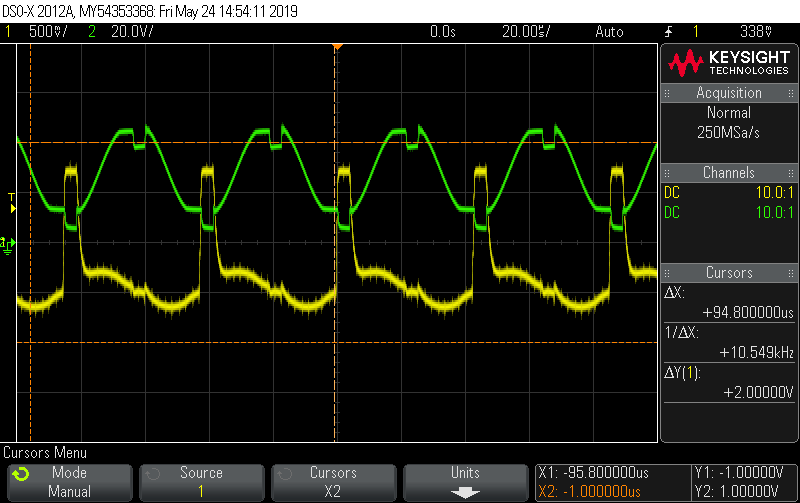
\includegraphics[width=.9\textwidth]{figures/scope_21.png}
\caption{In yellow the input 'TP2' to the power switch is shown and in green the output 'TP1' of the switch, controlling the transformer. The reference voltage has been increased to get the maximum high voltage output ($\SI{3759}{\volt}$).}
\label{fig:scope_21}
\end{figure}


\begin{figure}[H]
\centering
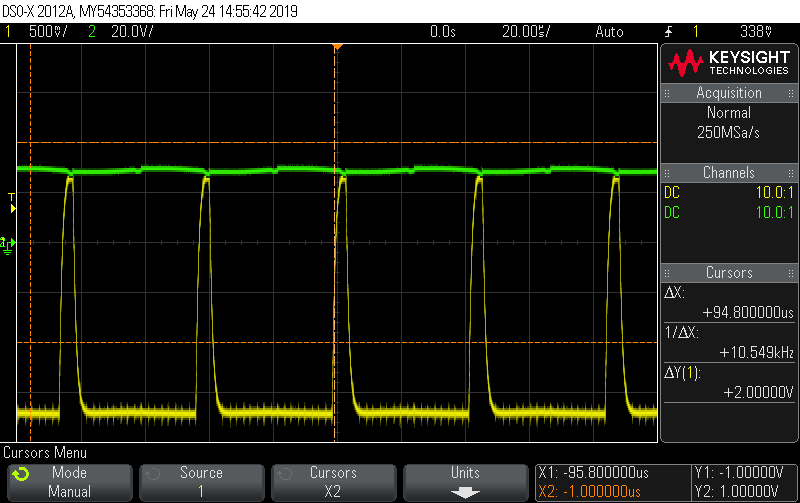
\includegraphics[width=.9\textwidth]{figures/scope_22.png}
\caption{In yellow the input 'TP2' to the power switch is shown and in green the output 'TP1' of the switch, controlling the transformer. The reference voltage has been decreased to get the minimum high voltage output ($\SI{157.7}{\volt}$).}
\label{fig:scope_22}
\end{figure}

